
\subsection{Participants} 
Protocol implementation involves realization of the protocol cryptographic building blocks as well as the means of data communication between them. Building blocks are placed at the following locations, which correspond to protocol participants:

\begin{itemize}%[label=$\bullet$]
	\item Citadel contract.
	\item User software.
	\item License provider software.
	\item Service provider software.
\end{itemize}

Data communication between protocol participants is realized by the following communication modes:

\begin{itemize}%[label=$\bullet$]
	\item Transaction changing the contract state.
	\item Query against the contract state
	\item Storing data directly in blockchain by issuing recipient-less transaction
	\item Retrieving data from blockchain by scanning transactions
\end{itemize}

The following diagram illustrates the interaction between protocol participants and indicates the communication means used.

\begin{figure}[h]
	\centering
		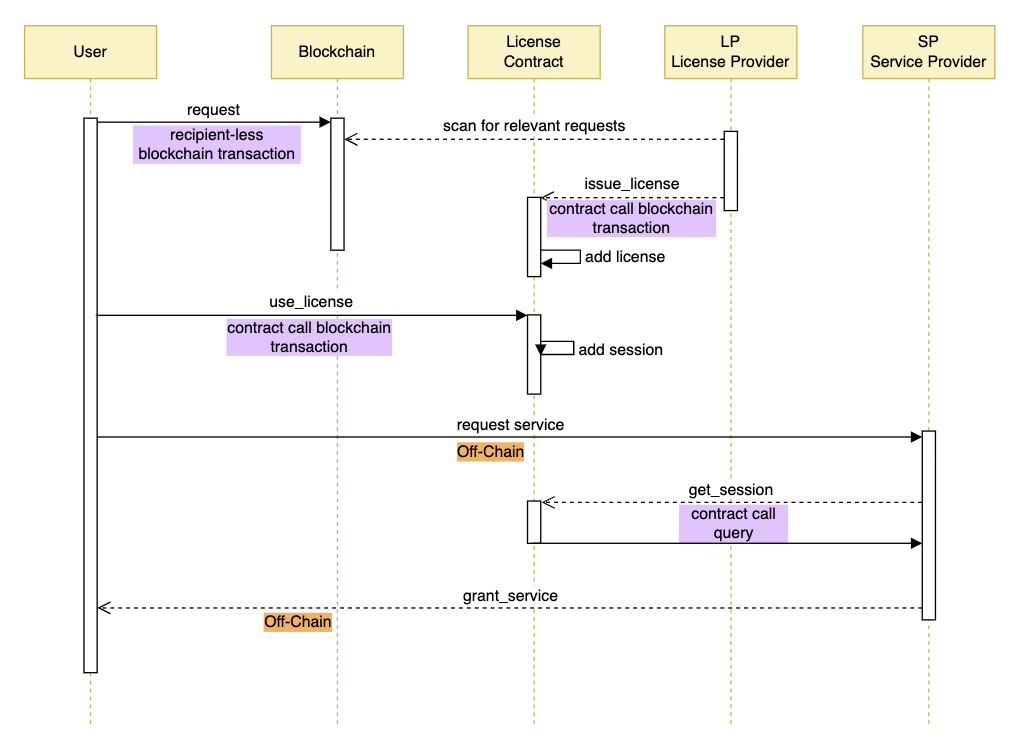
\includegraphics[width=390pt,draft=false]{images/implementation.png}
	\caption{Interaction between protocol participants}
	\label{fig:implementation}
\end{figure}


\subsection{License Contract}

License contract maintains state consisting of the following data:

\begin{itemize}%[label=$\bullet$]
	\item List of sessions.
	\item Map of licenses and their positions in the Merkle tree.
	\item Merkle tree of license hashes.
\end{itemize}


Contract provides the following methods:

\begin{itemize}%[label=$\bullet$]
	\item issue-license
	\item use-license
	\item get-session
\end{itemize}


\textit{issue-license} adds a license to a Merkle tree of licenses. \textit{use-license} attempts to verify the proof and, if verified, adds a new session to a list of sessions, nullifies the license in the Merkle tree. \textit{get-session} finds a session in a list of sessions and returns it to the caller.


